\documentclass[tikz,border=8pt]{standalone}
\usepackage{amsmath,amssymb}
\usetikzlibrary{arrows.meta,positioning,fit,shapes.geometric}
\definecolor{deepblue}{RGB}{26,58,99}
\definecolor{deepgreen}{RGB}{22,103,72}
\begin{document}
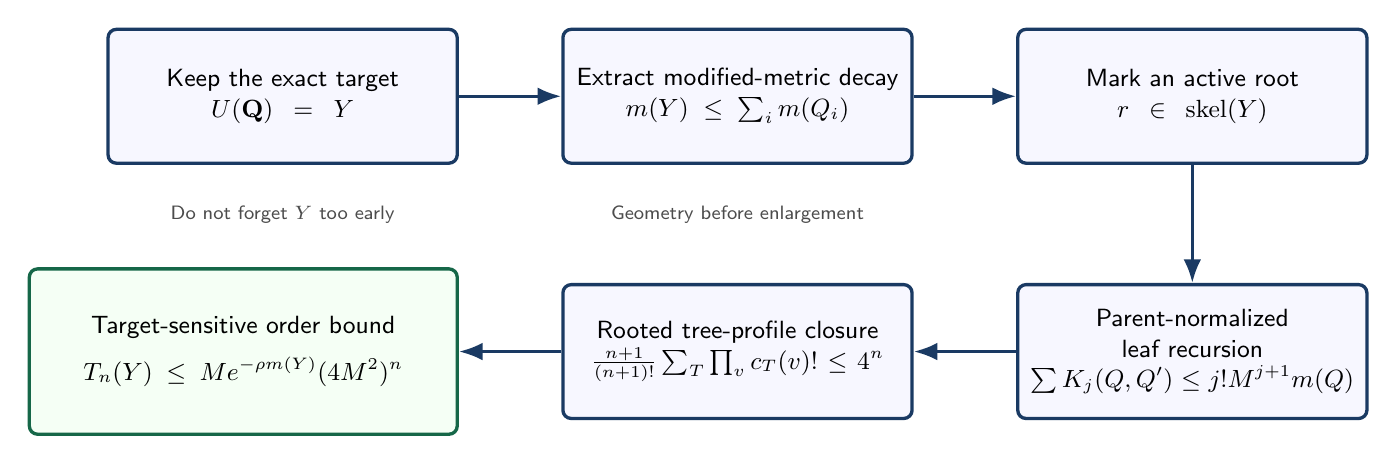
\begin{tikzpicture}[
  box/.style={draw=deepblue,very thick,rounded corners=3pt,fill=blue!3,align=center,minimum height=17mm,text width=42mm,font=\sffamily\small},
  result/.style={draw=deepgreen,very thick,rounded corners=3pt,fill=green!4,align=center,minimum height=21mm,text width=52mm,font=\sffamily\small},
  arr/.style={-{Latex[length=3mm]},very thick,deepblue},
  note/.style={font=\sffamily\scriptsize,align=center,text=black!70}
]
\node[box] (target) {Keep the exact target\\$U(\mathbf Q)=Y$};
\node[box,right=13mm of target] (stitch) {Extract modified-metric decay\\$m(Y)\le\sum_i m(Q_i)$};
\node[box,right=13mm of stitch] (root) {Mark an active root\\$r\in\operatorname{skel}(Y)$};
\node[box,below=15mm of root] (leaf) {Parent-normalized leaf recursion\\$\sum K_j(Q,Q')\le j!M^{j+1}m(Q)$};
\node[box,left=13mm of leaf] (trees) {Rooted tree-profile closure\\$\frac{n+1}{(n+1)!}\sum_T\prod_v c_T(v)!\le4^n$};
\node[result,left=13mm of trees] (out) {Target-sensitive order bound\\[2mm]$T_n(Y)\le M e^{-\rho m(Y)}(4M^2)^n$};
\draw[arr] (target) -- (stitch);
\draw[arr] (stitch) -- (root);
\draw[arr] (root) -- (leaf);
\draw[arr] (leaf) -- (trees);
\draw[arr] (trees) -- (out);
\node[note,below=4mm of target] {Do not forget $Y$ too early};
\node[note,below=4mm of stitch] {Geometry before enlargement};
\end{tikzpicture}
\end{document}
